\chapter{長期講習での利用を想定した時間割作成支援システム}
% create画面の説明 > execute画面の説明 > confilm画面の説明.
\section{システムの構成と新規講習ファイルの記載方法}
本研究で構築するシステムは,新規講習ファイル作成画面,担当割り振り探索画面,作成データ確認画面の3画面で構成される.新規講習ファイル作成画面では,時間割作成者がフォームに入力した情報をもとに,講習中における生徒情報と講師情報,および生徒と講師の相性を記載するための新規講習ファイルをExcel形式で出力する.新規講習ファイル作成画面を図\ref{s04041}に示す.担当割り振り探索画面では,入力済みの新規講習ファイルを読み込み,各生徒が受講する各授業の担当講師を決定した担当割り振りをExcel形式で出力する.担当割り振り探索画面を図\ref{s04043}に示す.作成データ確認画面では,同じ講習名の新規講習ファイルや担当割り振りの生成を防止するために,過去に生成した新規講習ファイルと担当割り振りを確認できる.作成データ確認画面を図\ref{s04044}に示す.

新規講習ファイルにおける講師の担当可能科目欄には,科目を講師が担当可能ならば1,担当不可能ならば0を入力する.生徒の受講可能日時と講師の勤務可能日時欄には,受講,勤務可能な日時ならば1,不可能な日時ならば0を入力する.また,生徒と講師の相性の欄には,生徒と講師の相性が良い組み合わせでは1,悪い組み合わせでは0を入力する.新規講習ファイルの入力例を図\ref{i04041}〜図\ref{i04045}に示す.

\begin{figure}[htbp]
\begin{center}
\includegraphics[scale=0.4]{image/create/04041.eps}
\caption{新規講習ファイル作成画面}
\label{s04041}
\end{center}
\end{figure}

\begin{figure}[htbp]
\begin{center}
\includegraphics[scale=0.4]{image/execute/04043.eps}
\caption{担当割り振り探査画面}
\label{s04043}
\end{center}
\end{figure}

\begin{figure}[htbp]
\begin{center}
\includegraphics[scale=0.4]{image/confirm/04044_1.eps}

    (a) 過去に生成した新規講習ファイル\\
\end{center}
\end{figure}

\begin{figure}[htbp]
\begin{center}
\includegraphics[scale=0.4]{image/confirm/04044_2.eps}

    (b) 過去に生成した担当割り振り\\
\caption{作成データ確認画面}
\label{s04044}
\end{center}
\end{figure}

\begin{figure}[htbp]
\begin{center}
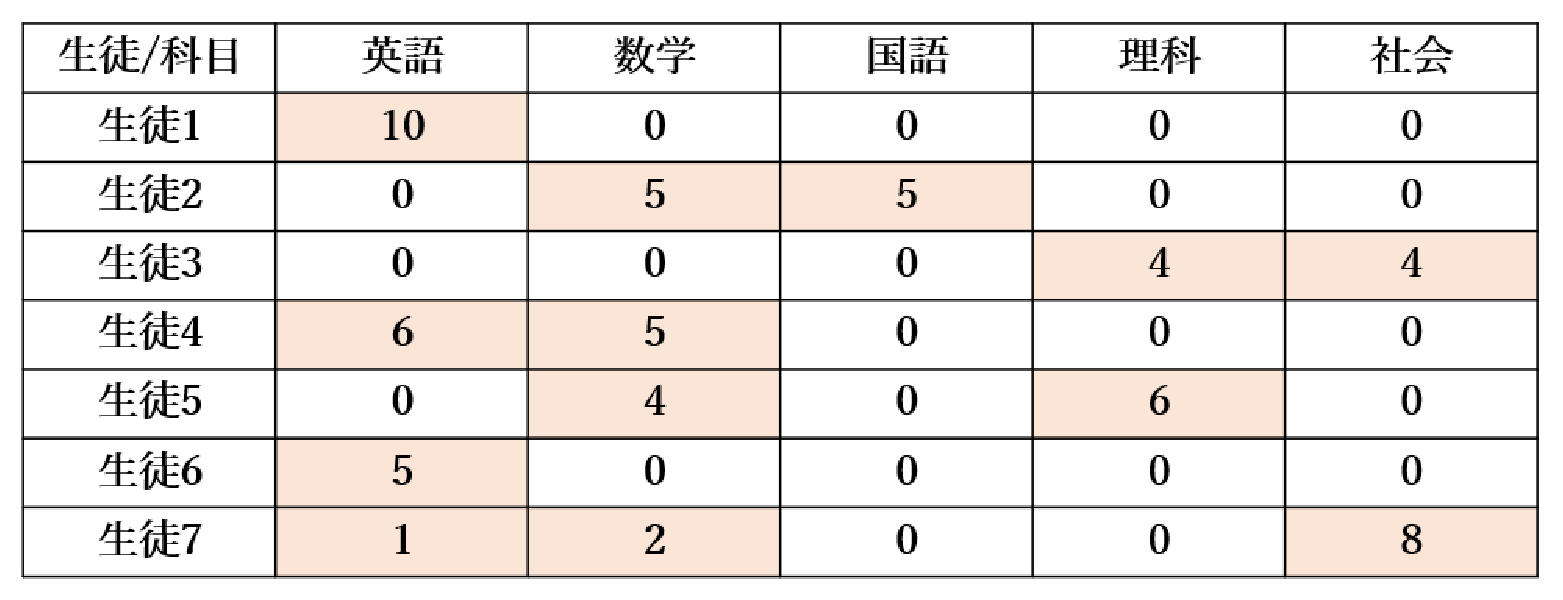
\includegraphics[scale=0.5]{image/new_file/04042_1.eps}
\caption{生徒の受講科目とコマ数の入力例}
\label{i04041}
\end{center}
\end{figure}

\begin{figure}[htbp]
\begin{center}
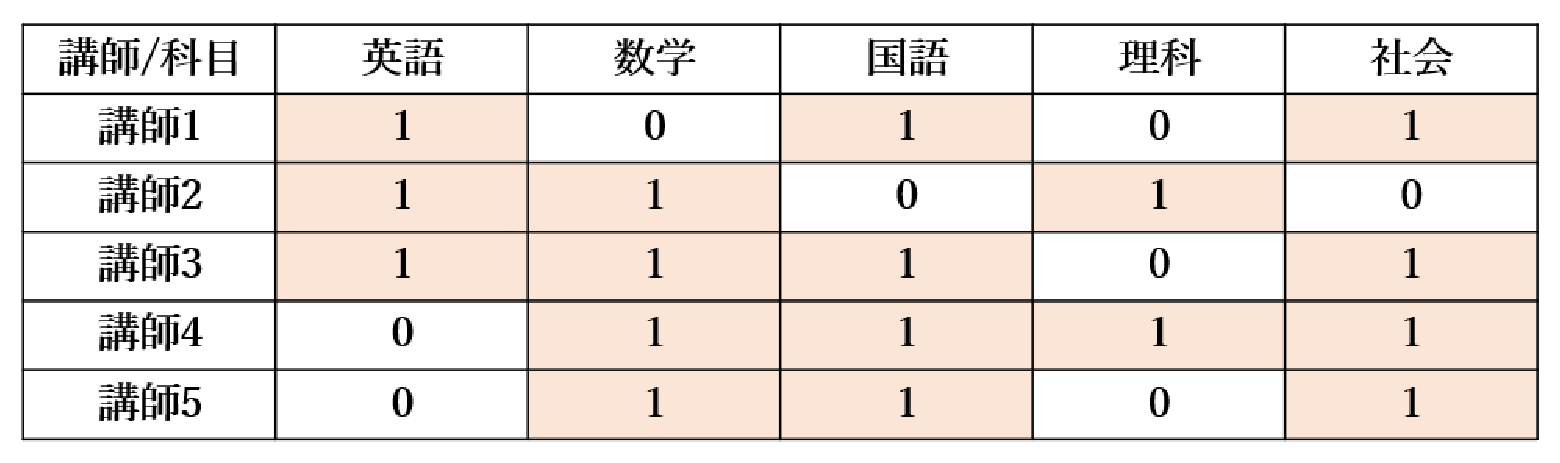
\includegraphics[scale=0.5]{image/new_file/04042_2.eps}
\caption{講師の担当可能科目の入力例}
\label{i04042}
\end{center}
\end{figure}

\begin{figure}[htbp]
\begin{center}
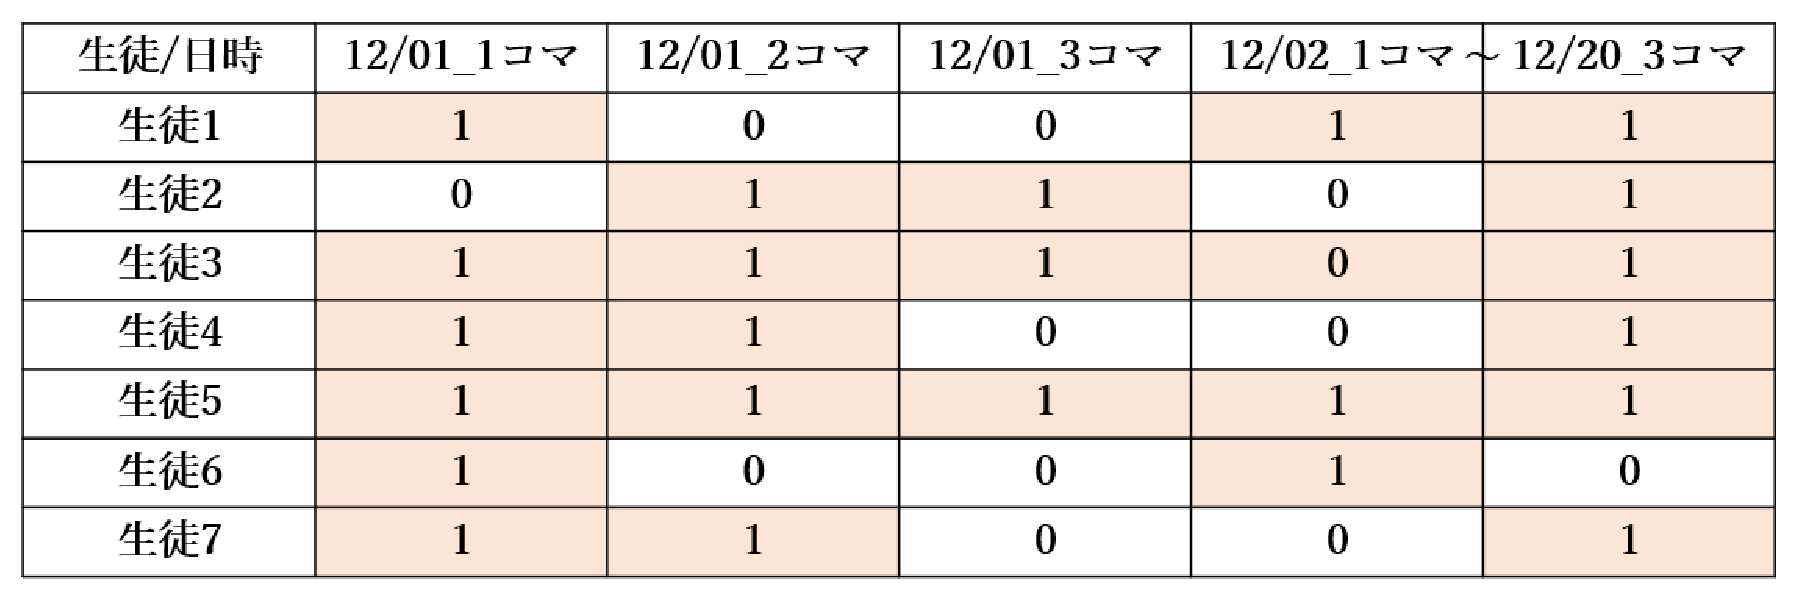
\includegraphics[scale=0.5]{image/new_file/04042_3.eps}
\caption{生徒の受講可能日時の入力例}
\label{i04043}
\end{center}
\end{figure}

\begin{figure}[htbp]
\begin{center}
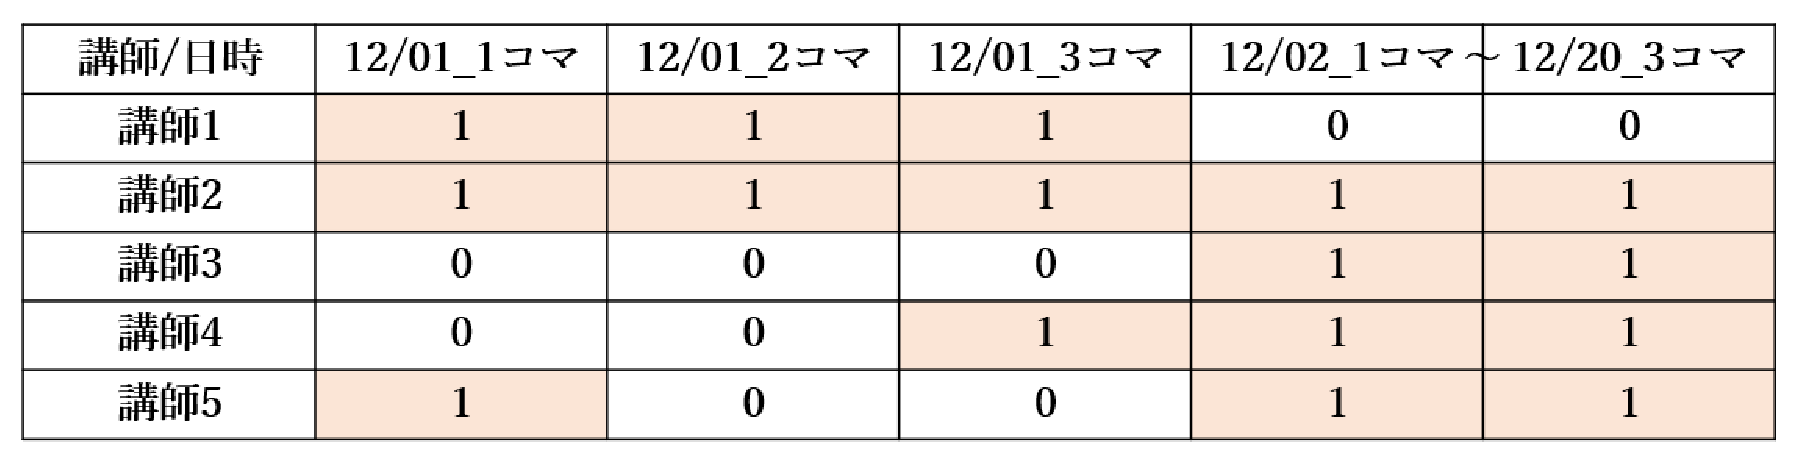
\includegraphics[scale=0.5]{image/new_file/04042_4.eps}
\caption{講師の勤務可能日時の入力例}
\label{i04044}
\end{center}
\end{figure}

\begin{figure}[htbp]
\begin{center}
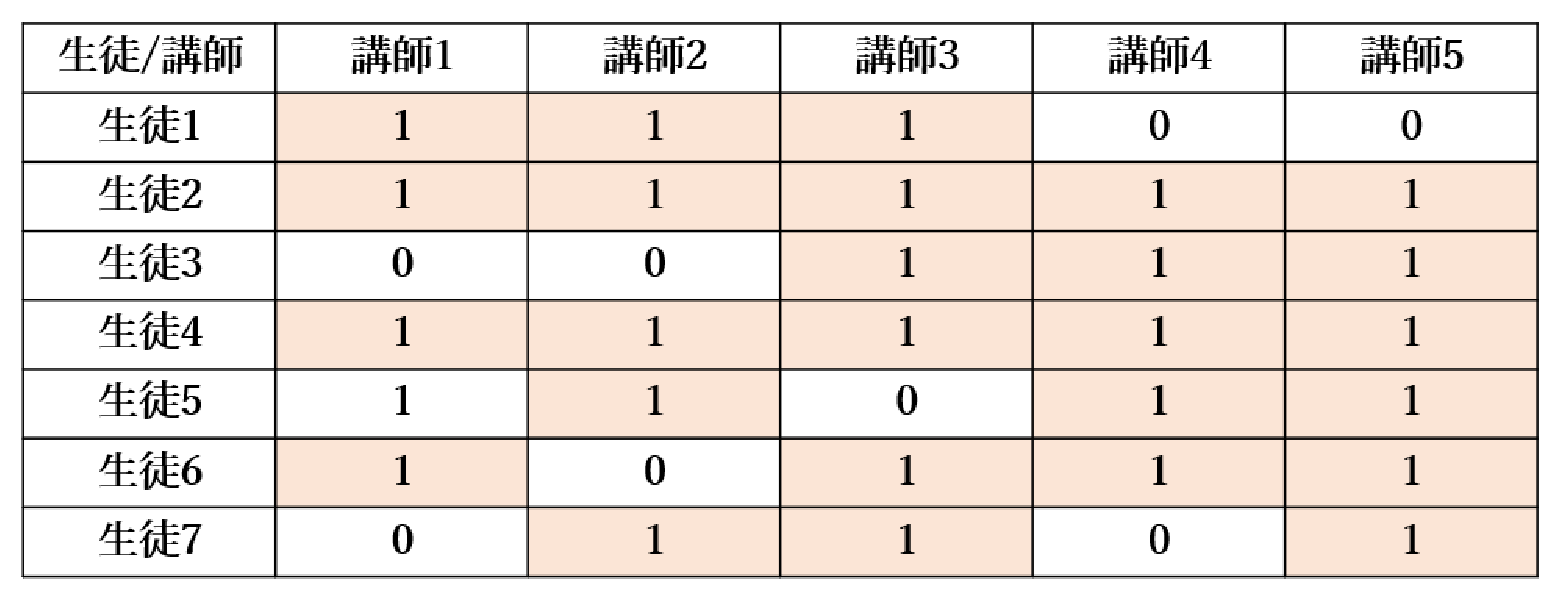
\includegraphics[scale=0.5]{image/new_file/04042_5.eps}
\caption{生徒と講師の相性の入力例}
\label{i04045}
\end{center}
\end{figure}
  
\section{担当割り振り決定手順}
生徒が希望する科目とコマ数,および講師の担当可能科目を考慮し,生徒の受講可能日時と講師の勤務可能日時の合致度が高く,講師ごとの勤務率にばらつきが少ない担当割り振りを決定するために
,GAを使用する.新規講習ファイルに入力した生徒情報,講師情報に不備がある場合,実行不可能であることを警告する.不備がない場合,一定回数の次世代生成後,最適解をExcelファイルに出力する.担当割り振りの出力例を図\ref{04045}に示す.

\begin{figure}[t]
\begin{center}
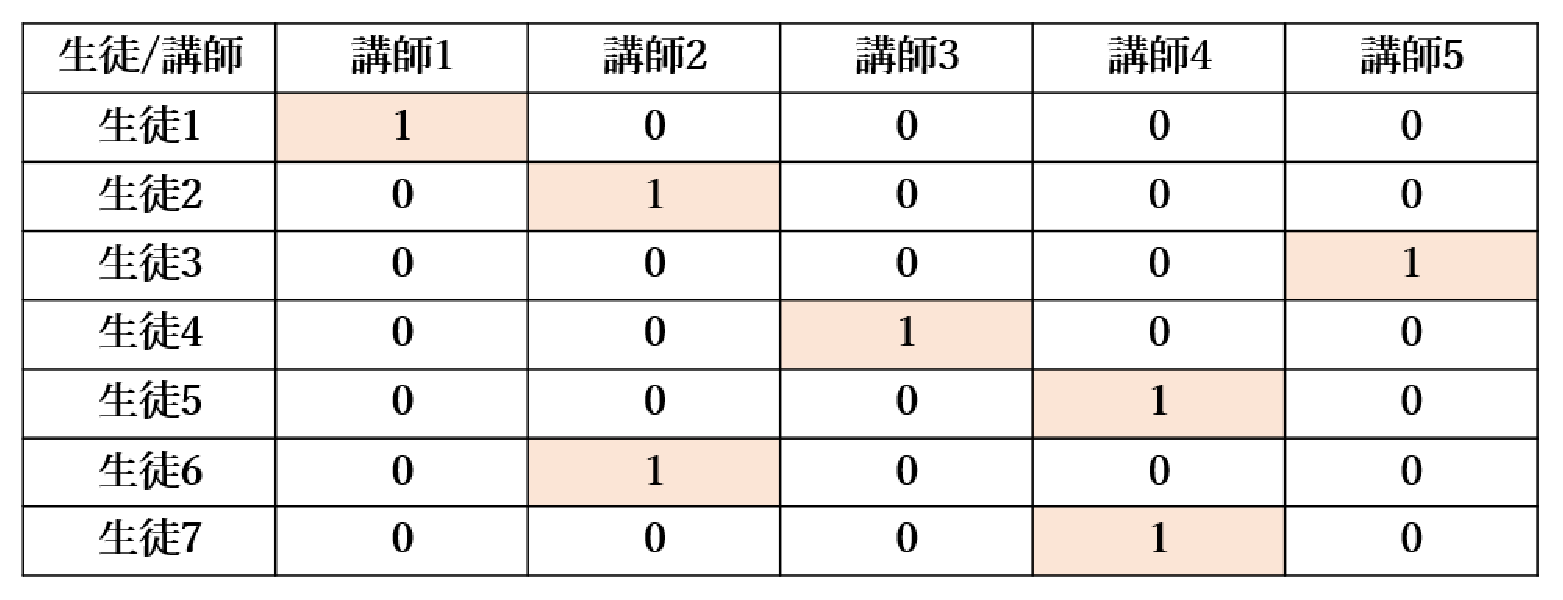
\includegraphics[scale=0.5]{image/new_file/04045.eps}
\caption{担当割り振り出力例}
\label{04045}
\end{center}
\end{figure}

\section{染色体と適応度}
全生徒の受講科目数の合計を$S$,講師数を$T$とし,染色体は$S×T$の2次元配列$chrom$で表す.全生徒の全受講科目に対して1〜$S$の番号を割り当てると,$chrom[i][j]$は科目$i$を講師$j$が担当するとき1,担当しないとき0となる.また,初期集団生成時に,講師が担当できない科目,および受講する生徒と講師の相性が悪い科目に対応する遺伝子を0にし,進化オペレータによって遺伝子の値を変化させないようにする.

本研究では,生徒の受講可能日時と講師の勤務可能日時の合致度が高く,各講師の勤務可能コマ数に対する勤務率が理想勤務率$\alpha$に近い担当割り振りほど高評価となるように適応度を算出する.科目$i$を受講する生徒と講師$j$の両者で都合の合うコマ数を$X$とし,講習中に実施されるコマ数を$E$としたとき,講習期間内における科目$i$を受
講する生徒の受講可能日時と講師$j$の勤務可能日時の合致度$MR_{ij}$は式\ref{00041}により算出される.

\begin{equation}
  \label{00041}
  MR_{ij}=\frac{chrom[i][j]×X}{E}
\end{equation}

また,全生徒と全講師の合致度の平均値$ave$と標準偏差$std$は式\ref{00042},\ref{00043}より算出される.

\begin{equation}
  \label{00042}
  % f_1=\sum_{k=1}^{n}\frac{v(m_k)}{b(m_k)-1}
  ave=\frac{\sum_{ij}MR_{ij}}{S}
\end{equation}

\begin{equation}
  \label{00043}
  std=\sqrt{ \frac{1}{S} \sum_{ij}\left(MR_{ij}-ave\right) }
\end{equation}

全生徒と全講師の合致度に関する評価値$f_{1}$は式\ref{00044}より算出される.

\begin{equation}
  \label{00044}
  f_{1}=\frac{1}{2}\left\{\left(\frac{1}{1+e^{-10(ave-0.5)}}\right)^5+\left(\frac{1}{1+e^{-10(std-0.5)}}\right)^5\right\}
\end{equation}

講師$j$の勤務可能コマ数を$WORK_{j}$,生徒$c$が希望する受講コマ数を$H_{c}$としたとき, $\alpha$は式\ref{00045}より算出される.

\begin{equation}
  \label{00045}
  \alpha =\frac{\sum_{c}H_{c}}{\sum_{j}WORK_{j}}
\end{equation}

また,講師$j$の勤務可能コマ数に対する勤務率$WR_{j}$は式\ref{00046}より算出される.

\begin{equation}
  \label{00046}
  WR_{j}=\frac{\sum_{i}chrom[i][j]}{WORK_{j}}
\end{equation}

各講師の勤務率と理想勤務率の平均二乗誤差を$rmse$とするとき,講師ごとの勤務率に関する評価値$f_{2}$は式\ref{00047}により算出される.

\begin{equation}
  \label{00047}
  f_{2}=\left(\frac{1}{1+e^{\log_{1.4}rmse}}\right)^{7}
\end{equation}

重み係数を$w$とするとき,解候補を評価する適応度$f$は式\ref{00048}で表される.
\begin{equation}
  \label{00048}
  f=wf_{1}+(1-w)f_{2}
\end{equation}

\section{交叉と選択}
より効果的な交叉手法と選択手法を調査するための予備実験を実施した.過去に実施された冬期講習情報に基づき,1点交叉,50点交叉,100点交叉,150点交叉,200点交叉,249点交叉,一様交叉をルーレット選択,トーナメント選択,ランキング選択の3つの選択手法で各5回ずつ担当割り振り探索を実行した.ただし,$w$は0.5,世代交代数は1000,個体数は200,突然変異確率は0.01とする.


\begin{table}[t]
\begin{center}

  % \caption{各最適解の適応度の平均値}
  % \label{table4.1}
  % \begin{tabular}{|l|c|c|c|} \hline
  % 交叉/選択  & ルーレット選択 & トーナメント選択 & ランキング選択   \\\hline 
  % 1点&0.07628&0.06825&0.07720\\\hline
  % 50点&0.10232&0.09724&0.09954\\\hline
  % 100点&0.11850&0.13202&0.13721\\\hline
  % 150点&0.21766&0.25166&0.24720\\\hline
  % 200点&0.35556&0.38088&0.35271\\\hline
  % 249点&0.48594&0.49864&0.47955\\\hline
  % 一様交叉&0.47712&0.49891&0.47911\\\hline
  % \end{tabular}

  % \caption{各最適解の適応度の標準偏差}
  % \label{table4.2}
  % \begin{tabular}{|l|c|c|c|} \hline
  % 交叉/選択  & ルーレット選択 & トーナメント選択 & ランキング選択  \\\hline 
  % 1点     & 0.01911       & 0.00443      & 0.00401  \\\hline
  % 50点    & 0.00936       & 0.06860      & 0.01194  \\\hline
  % 100点   & 0.02987       & 0.01972      & 0.01004  \\\hline
  % 150点   & 0.01802       & 0.01186      & 0.02894  \\\hline
  % 200点   & 0.01169       & 0.01604      & 0.02561  \\\hline
  % 249点   & 0.00269       & 0.00056      & 0.00345  \\\hline
  % 一様交叉  & 0.00743       & 0.00071      & 0.00518  \\\hline
  % \end{tabular}
  % \begin{tabular}{|c|c|c|c|c|c|c|} \hline
  %   & \multicolumn{2}{|c|}{RC1}       & \multicolumn{2}{|c|}{RC2} & \multicolumn{2}{|c|}{RC3}\\\hline
  %   質問  & \MARU{1} & \MARU{2}             &  \MARU{1} & \MARU{2}      & \MARU{1}       & \MARU{2} \\\hline
  %   A     & 4        & 4        & 4         & 5                         & 4              & 5        \\\hline
  %   B     & 5        & 5        & 5         & 5                         & 5              & 5        \\\hline
  % \end{tabular}
  \caption{各最適解の適応度の平均値と標準偏差}
  \label{table4.1}
  % \begin{tabular}{|l|c|c|c|c|c|c|} \hline
  %   交叉/選択&\multicolumn{2}{|c|}{ルーレット選択}&\multicolumn{2}{|c|}{ルーレット選択}&\multicolumn{2}{|c|}{ランキング選択}\\\hline
  %   &平均値&標準偏差&平均値&標準偏差&平均値&標準偏差\\\hline
  %     1点&0.07628&0.01911&0.06825&0.00443&0.07720&0.00401\\\hline
  %    50点&0.10232&0.00936&0.09724&0.06860&0.09954&0.01194\\\hline
  %   100点&0.11850&0.02987&0.09724&0.01972&0.13721&0.01004\\\hline
  %   150点&0.21766&0.01802&0.25166&0.01186&0.24720&0.02894\\\hline
  %   200点&0.35556&0.01169&0.38088&0.01604&0.35271&0.02561\\\hline
  %   249点&0.48594&0.00269&0.49864&0.00056&0.47955&0.00345\\\hline
  %   一様交叉&0.47712&0.00743&0.49891&0.00071&0.47911&0.00518\\\hline
  % \end{tabular}
  \begin{tabular}{|l|c|c|c|c|c|c|} \hline
      交叉/選択&\multicolumn{2}{|c|}{ルーレット選択}&\multicolumn{2}{|c|}{トーナメント選択}&\multicolumn{2}{|c|}{ランキング選択}\\\hline
      &平均値&標準偏差&平均値&標準偏差&平均値&標準偏差\\\hline
      \ \ \:\:1点&0.0763&0.0191&0.0683&0.0044&0.0772&0.0040\\\hline
      \ \:50点&0.1023&0.0094&0.0972&0.0686&0.0995&0.0119\\\hline
      100点&0.1185&0.0299&0.0972&0.0197&0.1372&0.0100\\\hline
      150点&0.2177&0.0180&0.2517&0.0119&0.2472&0.0289\\\hline
      200点&0.3556&0.0117&0.3809&0.0160&0.3527&0.0256\\\hline
      249点&0.4859&0.0027&0.4986&0.0006&0.4796&0.0035\\\hline
      一様交叉&0.4771&0.0074&0.4989&0.0007&0.4791&0.0052\\\hline
    \end{tabular}

\end{center}
\end{table}

各最良個体の適応度の平均値と標準偏差を表\ref{table4.1}に示す.一様交叉とトーナメント選択の組み合わせで最も高い適応度が得られた.また,標準偏差も十分小さいことから,交叉手法は一様交叉,選択手法はトーナメント選択を採用する.